\documentclass[10pt]{article}
\usepackage{graphicx}
\usepackage{hyperref}
\usepackage{todonotes}

\title{Demographic Inclusiveness in Human Cell Studies}

\begin{document}
\maketitle
  
\section{Introduction}
  
The research process for preclinical studies typically progresses from cell models, to animal models, and finally human models. During the cell model stage, donors provide a sample of cells to be grown in a lab environment. The possibility of demographic bias in cell culture studies specifically the gender, age and ethnicity of human donors supplying the cells used for research can have significant consequences for the validity of findings in early-stage pharmaceutical studies. However, US federal regulations require broad spectrum representation of gender, age and ethnicity only during the final phase of clinical testing, the human model stage. What happens in the first phase of cell models is not regulated and can result in demographic bias. The question this study will address is what criteria biologists use when selecting cell sources for early studies and the research objective is to investigate whether there are quantifiable biases in extant literature for cell model studies.

The human genome's major structures recur across the global population regardless of geographical ancestry, self-identified race or sociocultural considerations \cite{xie2001molecular, cooper2003race}. Still, comparatively minor genetic variants generate predictable alterations in the therapeutic impact of some pharmaceutical treatments. Clustering patients by genotype can inform the course of drug therapies during treatment of cancer and organ transplant \cite{krynetski2000genetic, higashi2002association}. Because of these implications, the US Food and Drug Administration (FDA) recognized that genetic factors sensitize pharmaceutical efficacy and implemented the \textit{Demographic Rule} in 1998 which standardizes race and ethnicity representation during clinical trails based on the target therapeutic population identified by the drug's sponsor.

A study published in \textit{Science} showed that racial and ethnic diversity serves as an unsubstantiated proxy for broad spectrum representation of genetic variants during clinical trials \cite{haga2003fda}. A retrospective of the FDA's review of clinical trail protocols identified 10\% of the 185 products approved from 1995-1999 disclosed racial differences in the performance of the product on the label \cite{evelyn2001participation}. The same study showed that the clinical trials from the same period disclosed the participants' racial composition for 53\% of the nearly 500k individuals enrolled. Of the 260k participants for whom race was specified, white was most common (88\%), African American was comparable to US population percentage (8\%), and the report classified Hispanics as underrepresented, comprosing 1\% of participants.

Demographic bias in clinical trials is important and has been featured in leading journals such as \textit{Science} and \textit{Nature}. However, demographic bias in cell models remains a mystery and poses an interesting question deserving more thurough review. Not only could results of this study be published in previously mentioned prestigious journals, but it could also have a broader impact to enhance knowledge about inefficiencies in drug discovery processes and raise questions leading to extension of the FDA's Demographic Rule to the cell models phase. The proposed work aligns with current efforts to vet the efficacy and toxicity of drug candidates early in the discovery process and the intellectual merit of the proposed research lies in expanding the decision criteria for cell sources during the discovery process for an abridged implementation of personalized medicine.

\section{Data}

To systematically address the questions posed above, we adopt an developed and anlyzed a corpus of biomedical research publications from peer-reviewed sources. The dataset consists of 36,056 English-language full text papers selected from the \textsc{medline} database\footnote{\url{www.nlm.nih.gov/bsd/pmresources.html}.} using \textit{Medical Subject Headings} (MeSH) terms related to stem cell research. The text of the selected papers, downloaded from Scopus\footnote{\url{www.scopus.com}.} and PubMed Central\footnote{\url{www.ncbi.nlm.nih.gov/pmc}.}, and were tagged as papers working with \textit{stem cells}. Each full text paper in the dataset has an array of associated metadata such as publication date, venue, authorship, affiliation, etc.. This data will allow us to explore distribution of papers over time (see Figure \ref{dist1}) as well as other dimensions, like publication venue and author affiliations. More than 95\% of papers in our dataset were published after 2000 and is complete until about Q2 2014. Looking at the distribution of papers per country of origin for the journal in which they were published, we find a bias towards journals from the US which comprise about 50\% of all papers (Figure \ref{dist2}).

\begin{figure}[b!]
\centering
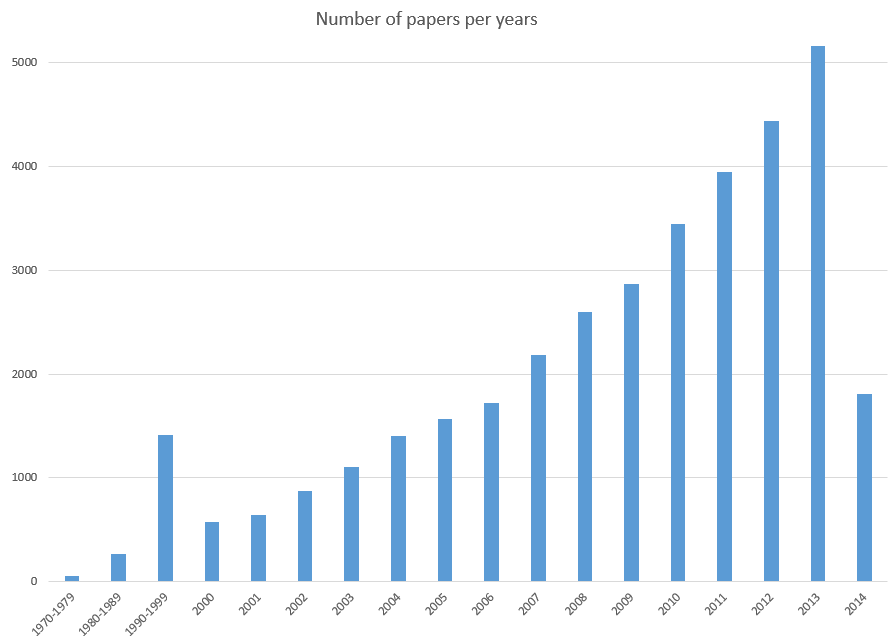
\includegraphics[width=0.98\columnwidth]{Figures/Figure1.png}
\caption{\label{dist1}Distribution of papers per year.}
\end{figure}

\begin{figure}[h!]
\centering
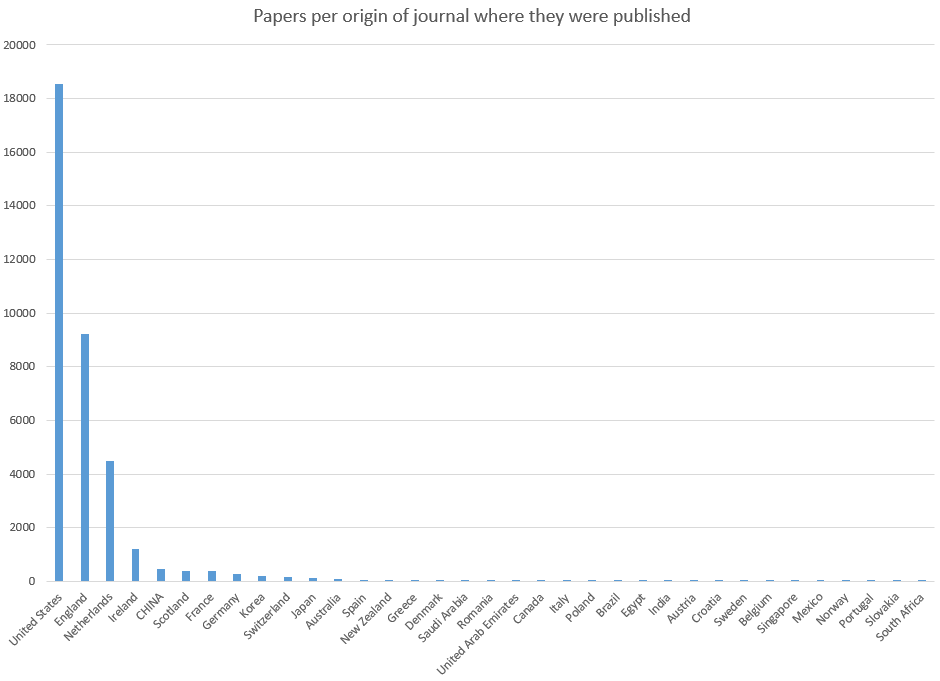
\includegraphics[width=0.98\columnwidth]{Figures/Figure2.png}
\caption{\label{dist2}Distribution of papers per country origin of journal.}
\end{figure}

\section{Initial results}
The source of human cells is either (1) primary or (2) cell lines. Primary cells are provided directly by a hospitalized patient. Outside the body, cell lose functionality and variations from parent to daughter cell increase. Therefore, primary cells have limited longevity and high genetic variability which can complicate comparisons with peer studies. Cell lines are better suited to peer-to-peer comparison because they offer a phenotypic standard. Cell lines begin as primary cells and are genetically modified to ensure intergenerational stability. The initial donor for most cell lines is specified in published literature whereas the donor for primary cell models varies based on the source, often disclosed at the discretion of the editor at the time of publication.

Our initial demographic characterizations are focused on cell lines, the distributors of which provide keywords for text search. This enables queries using the Web of Science and US Patent and Trademark Office databases. The demographics of the initial donor for most cell lines can be found in peer reviewed literature.

A database of 255 unique cell line designations and donor demographics is populated from commercial cell line repositories specification sheets and published literature. The cell line designation serves as query keywords to identify the most common cell lines used in the article database. Of the 255 unique cell lines, 137 cell lines were cited in at least 10 publications in our dataset\todo{AG: Why a min doc count?}. Figure \ref{pc3} presents the gender and ethnicity of the initial donor for the 137 most popular human cell lines in the the article dataset. Of the most commonly used cell lines, male donors are the majority, followed by female but with a significant proportion unspecified in the commercial repository's inventory description. A majority of the donors are either Caucasian or unspecified: combined, Asian and Black donors comprise 11\% of the available cell lines used a minimum of 10 times in the 36,056 publications.

\begin{figure}[h!]
\centering
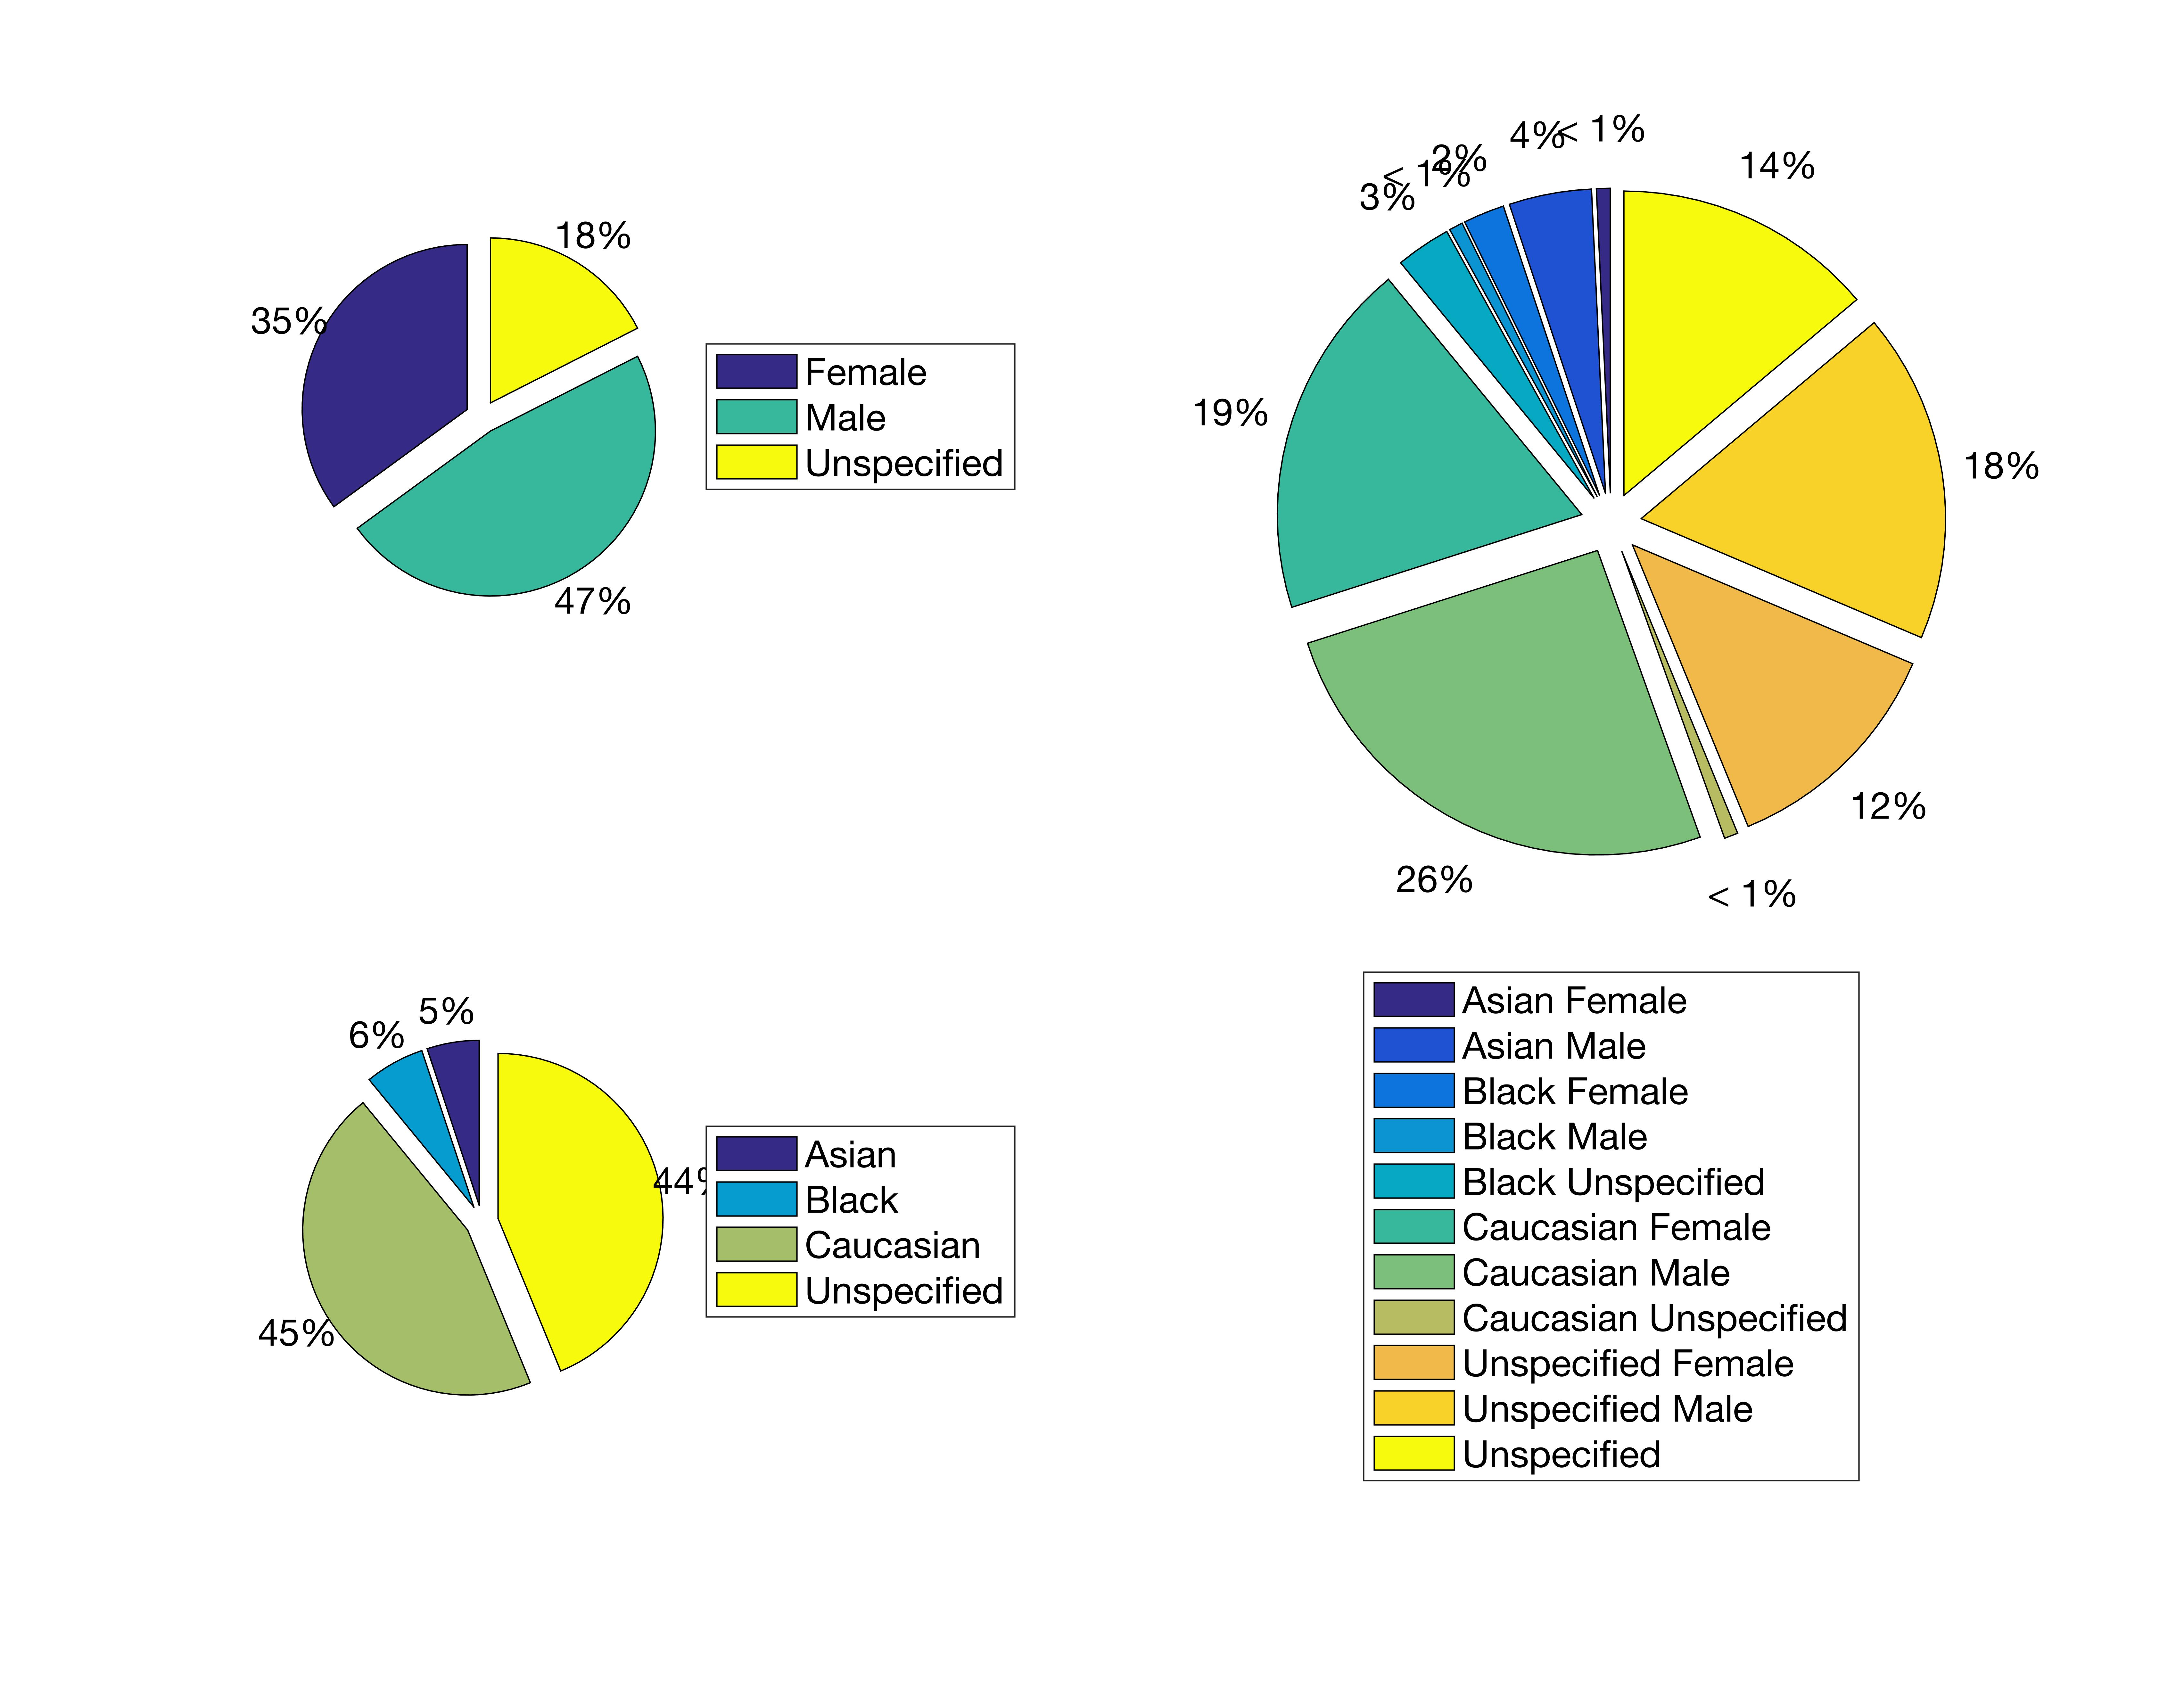
\includegraphics[width=0.98\columnwidth]{Figures/PieChart_3}
\caption{\label{pc3}Gender and ethnicity of initial donor for most popular human cell lines used in the article dataset.}
\end{figure}

The donor age for the 137 human cell line is shown in Figure \ref{sc1}. The mean donor age is 40.3 +/-25.4 years old. The mean for female and male donor cell lines are 37.3 +/-27.0 and 42.5 +/-24.1 years old respectively. Cell lines from Asian, Black and Caucasian donor ages averaged 45.8 +/-10.2, 20.8 +/-14.1, and 41.7 +/-25.8 years old respectively. 

\begin{figure}[h!]
\centering
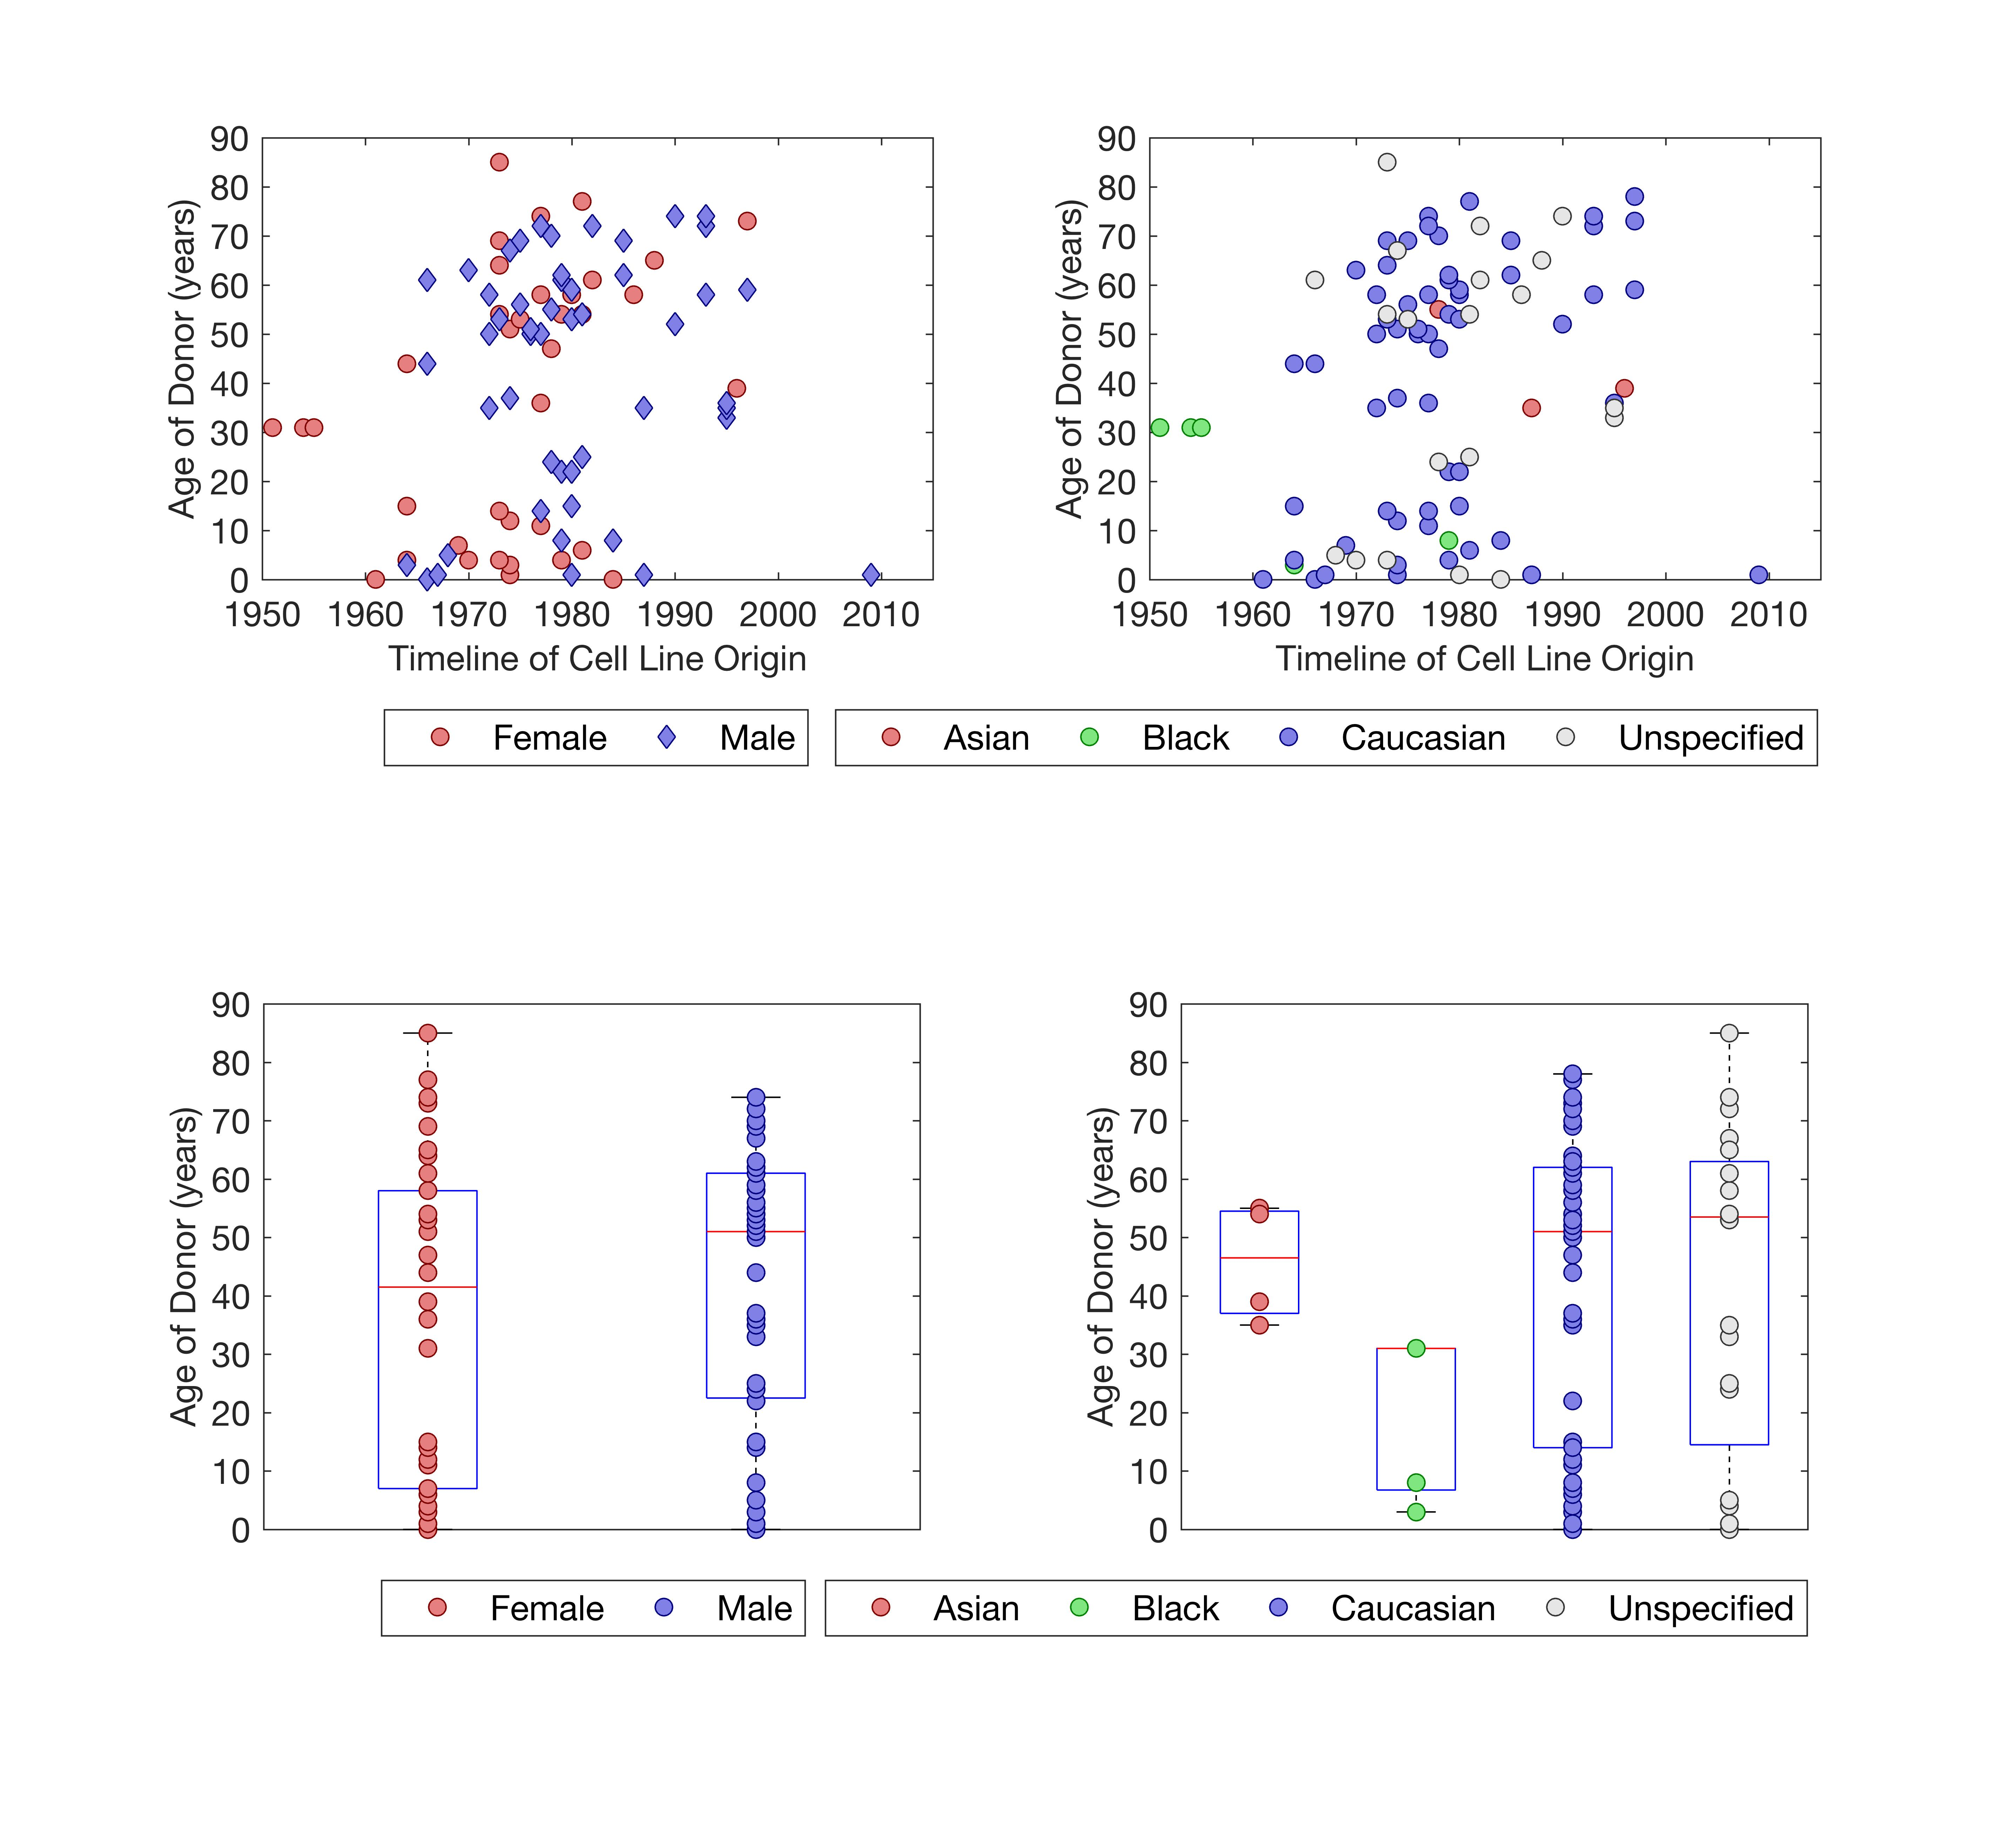
\includegraphics[trim={20cm 20cm 20cm 20cm}, width=0.98\columnwidth]{Figures/ScatterAge_2}
\caption{\label{sc1}Timeline of cell line introduction from 1951 to present, subdivided by donor age, gender and ethnicity.}
\end{figure}

\newpage
Figure \ref {pc1} presents the usage of cell lines in the article dataset and in patents in US Patent database. Both the article dataset and US patent database tend to use cell lines originating from Caucasian and female donors. \todo{AG: Should explain this Patents data: how were the cell lines found?}

\begin{figure}[h!]
\centering
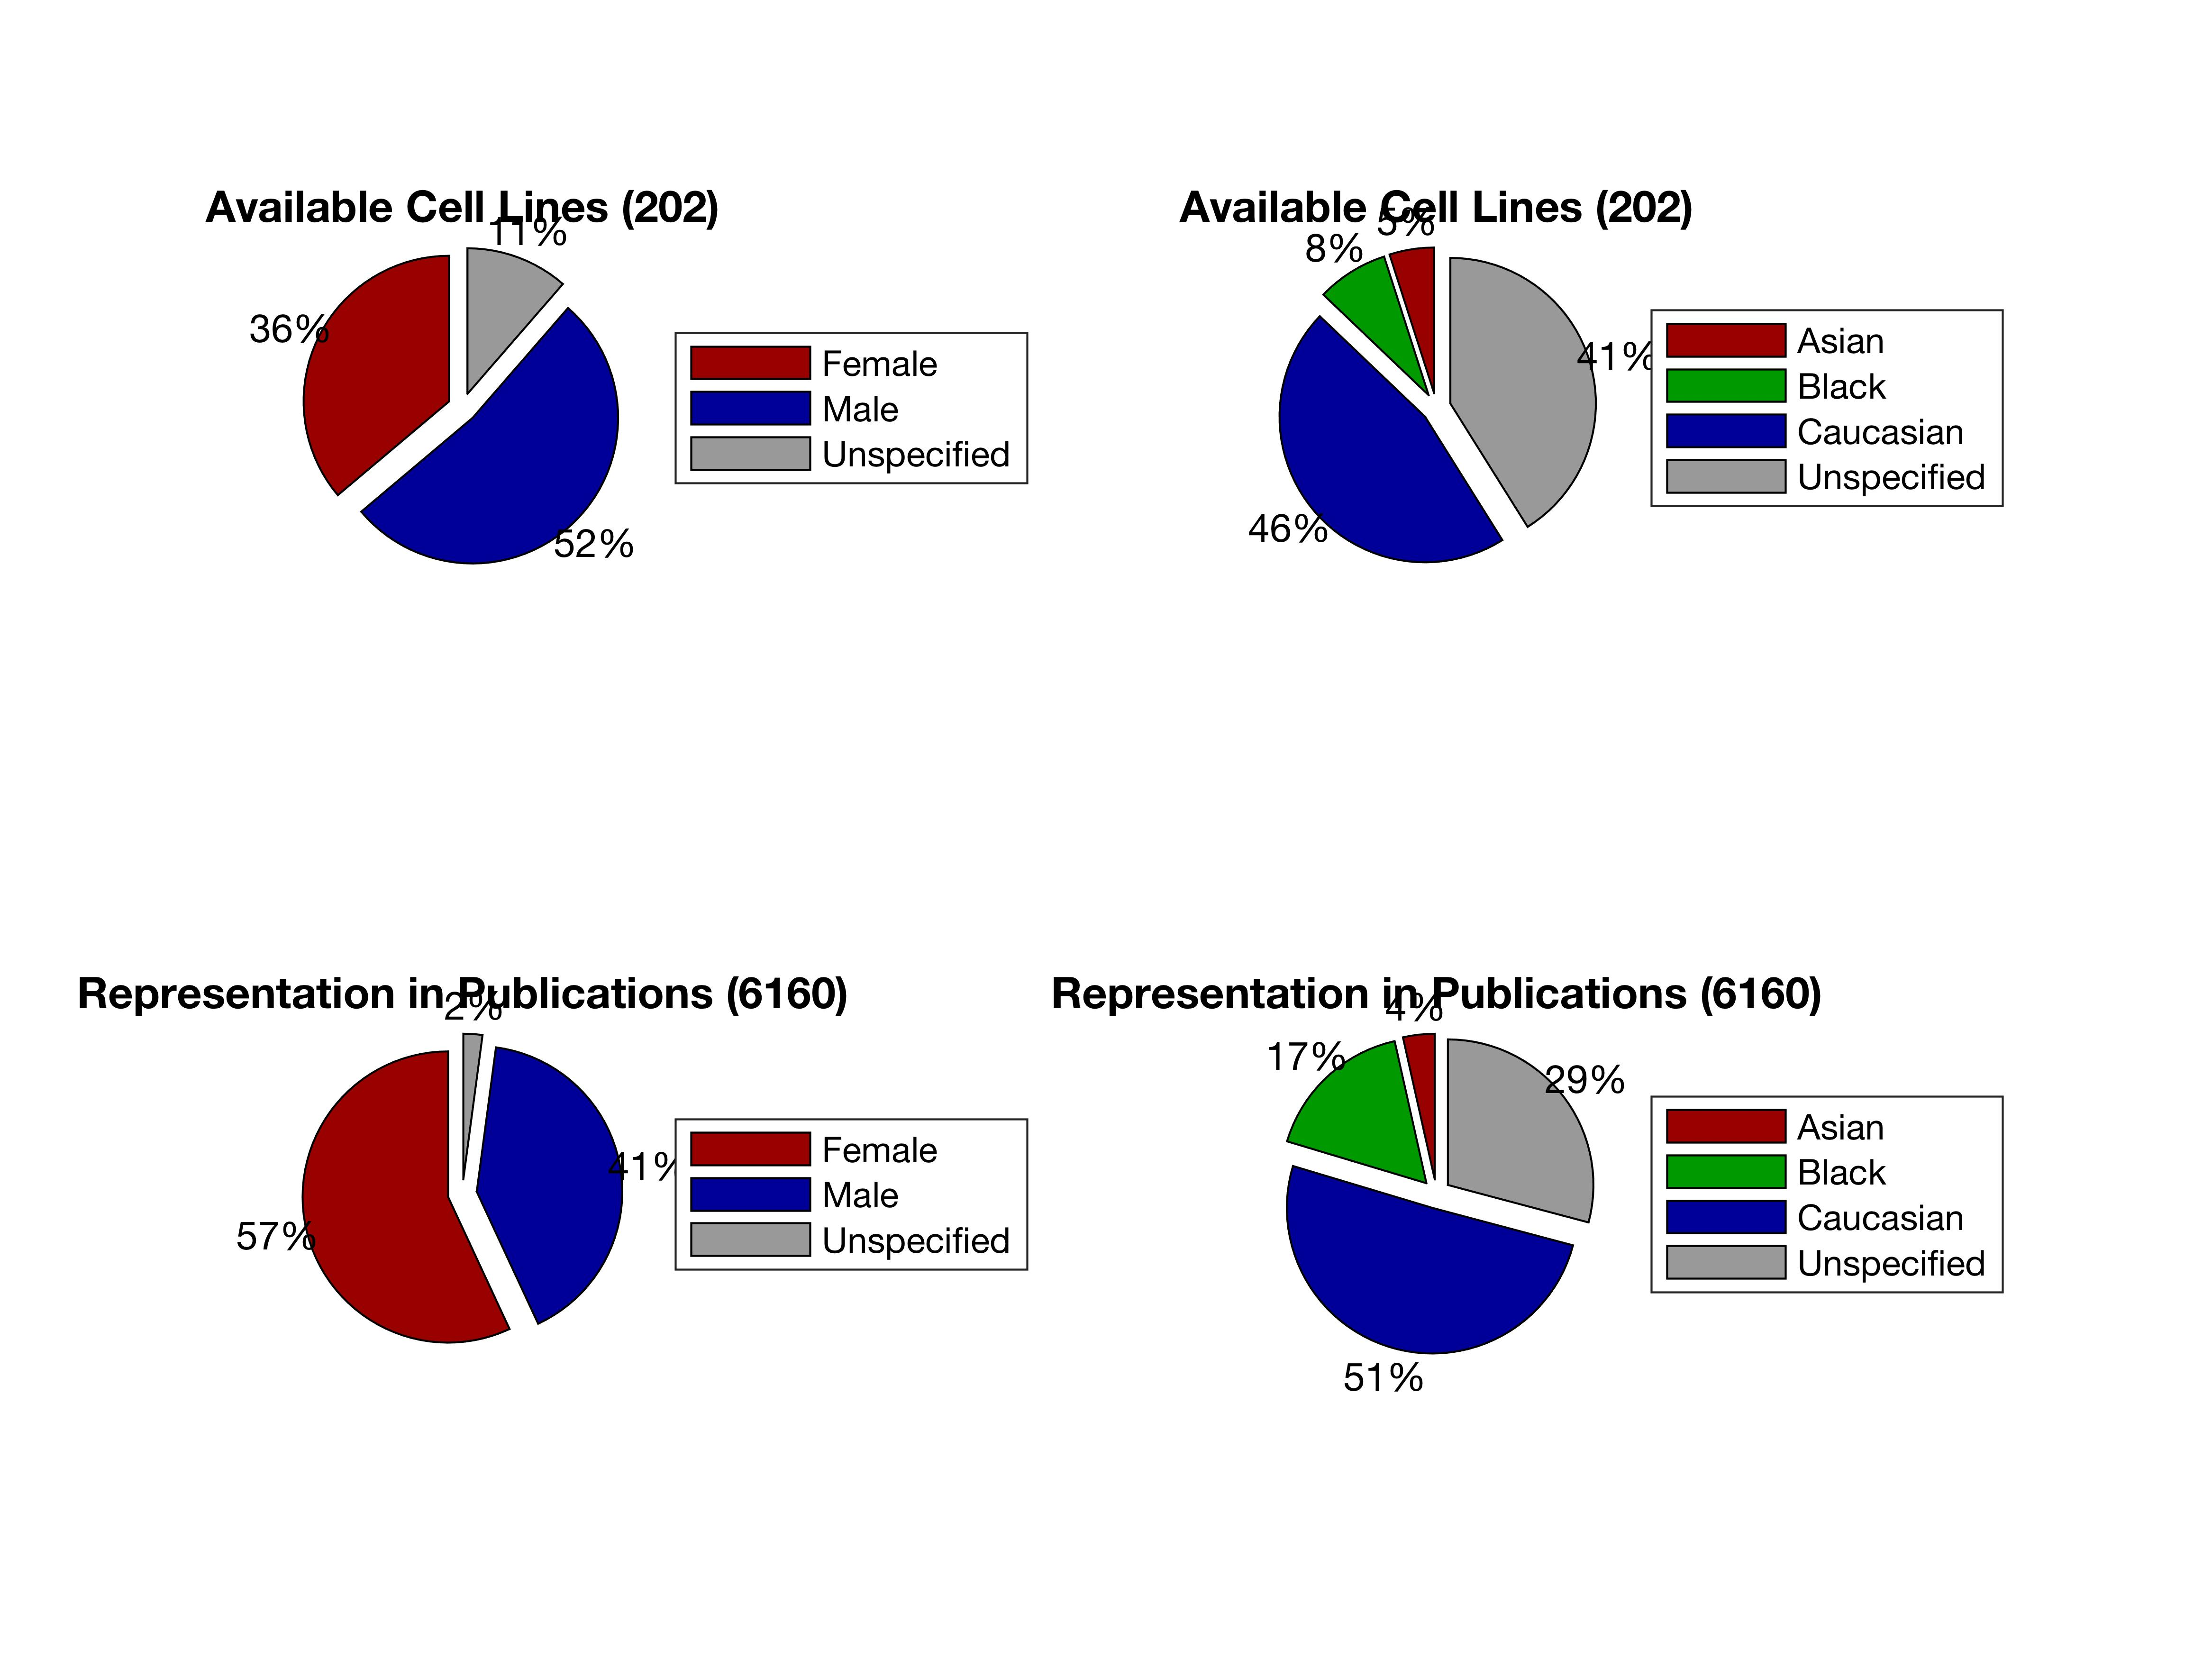
\includegraphics[width=0.79\columnwidth]{Figures/PieChart1}
\caption{\label{pc1} Comparison of gender and ethnicity representation of cell lines in our publication dataset and that resulting from queries to the US Patent database.}
\end{figure}

Figure \ref{pc2} divides the information in Figure \ref{pc1} into research topics: brain, breast cancer, colon/prostate, leukemia/lymphoma, kidney/bladder, and reproduction. The article dataset and patent database identified the same most abundant donor demographics for all research topics. There was strong agreement between the article dataset and the US patent database for demographic bias exists in breast cancer and kidney/bladder research. In other topics, there was considerably weaker agreement in the demographic profile of cell lines. 

\begin{figure}[h!]
\centering
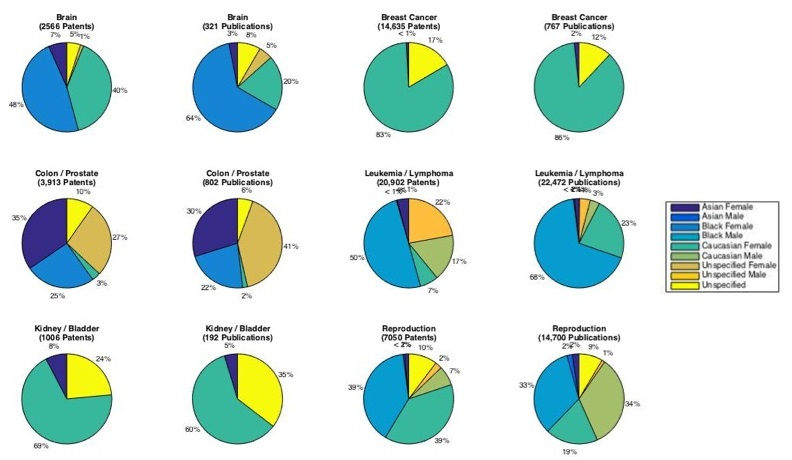
\includegraphics[width=0.98\columnwidth]{Figures/PieChart_2}
\caption{\label{pc2}Demographic profile of cell lines in the article dataset and in US patents data queried for research subjects: brain, breast cancer, colon/prostate, leukemia/lymphoma, kidney/bladder, and reproduction.}
\end{figure}


\begin{figure}[h!]
\centering
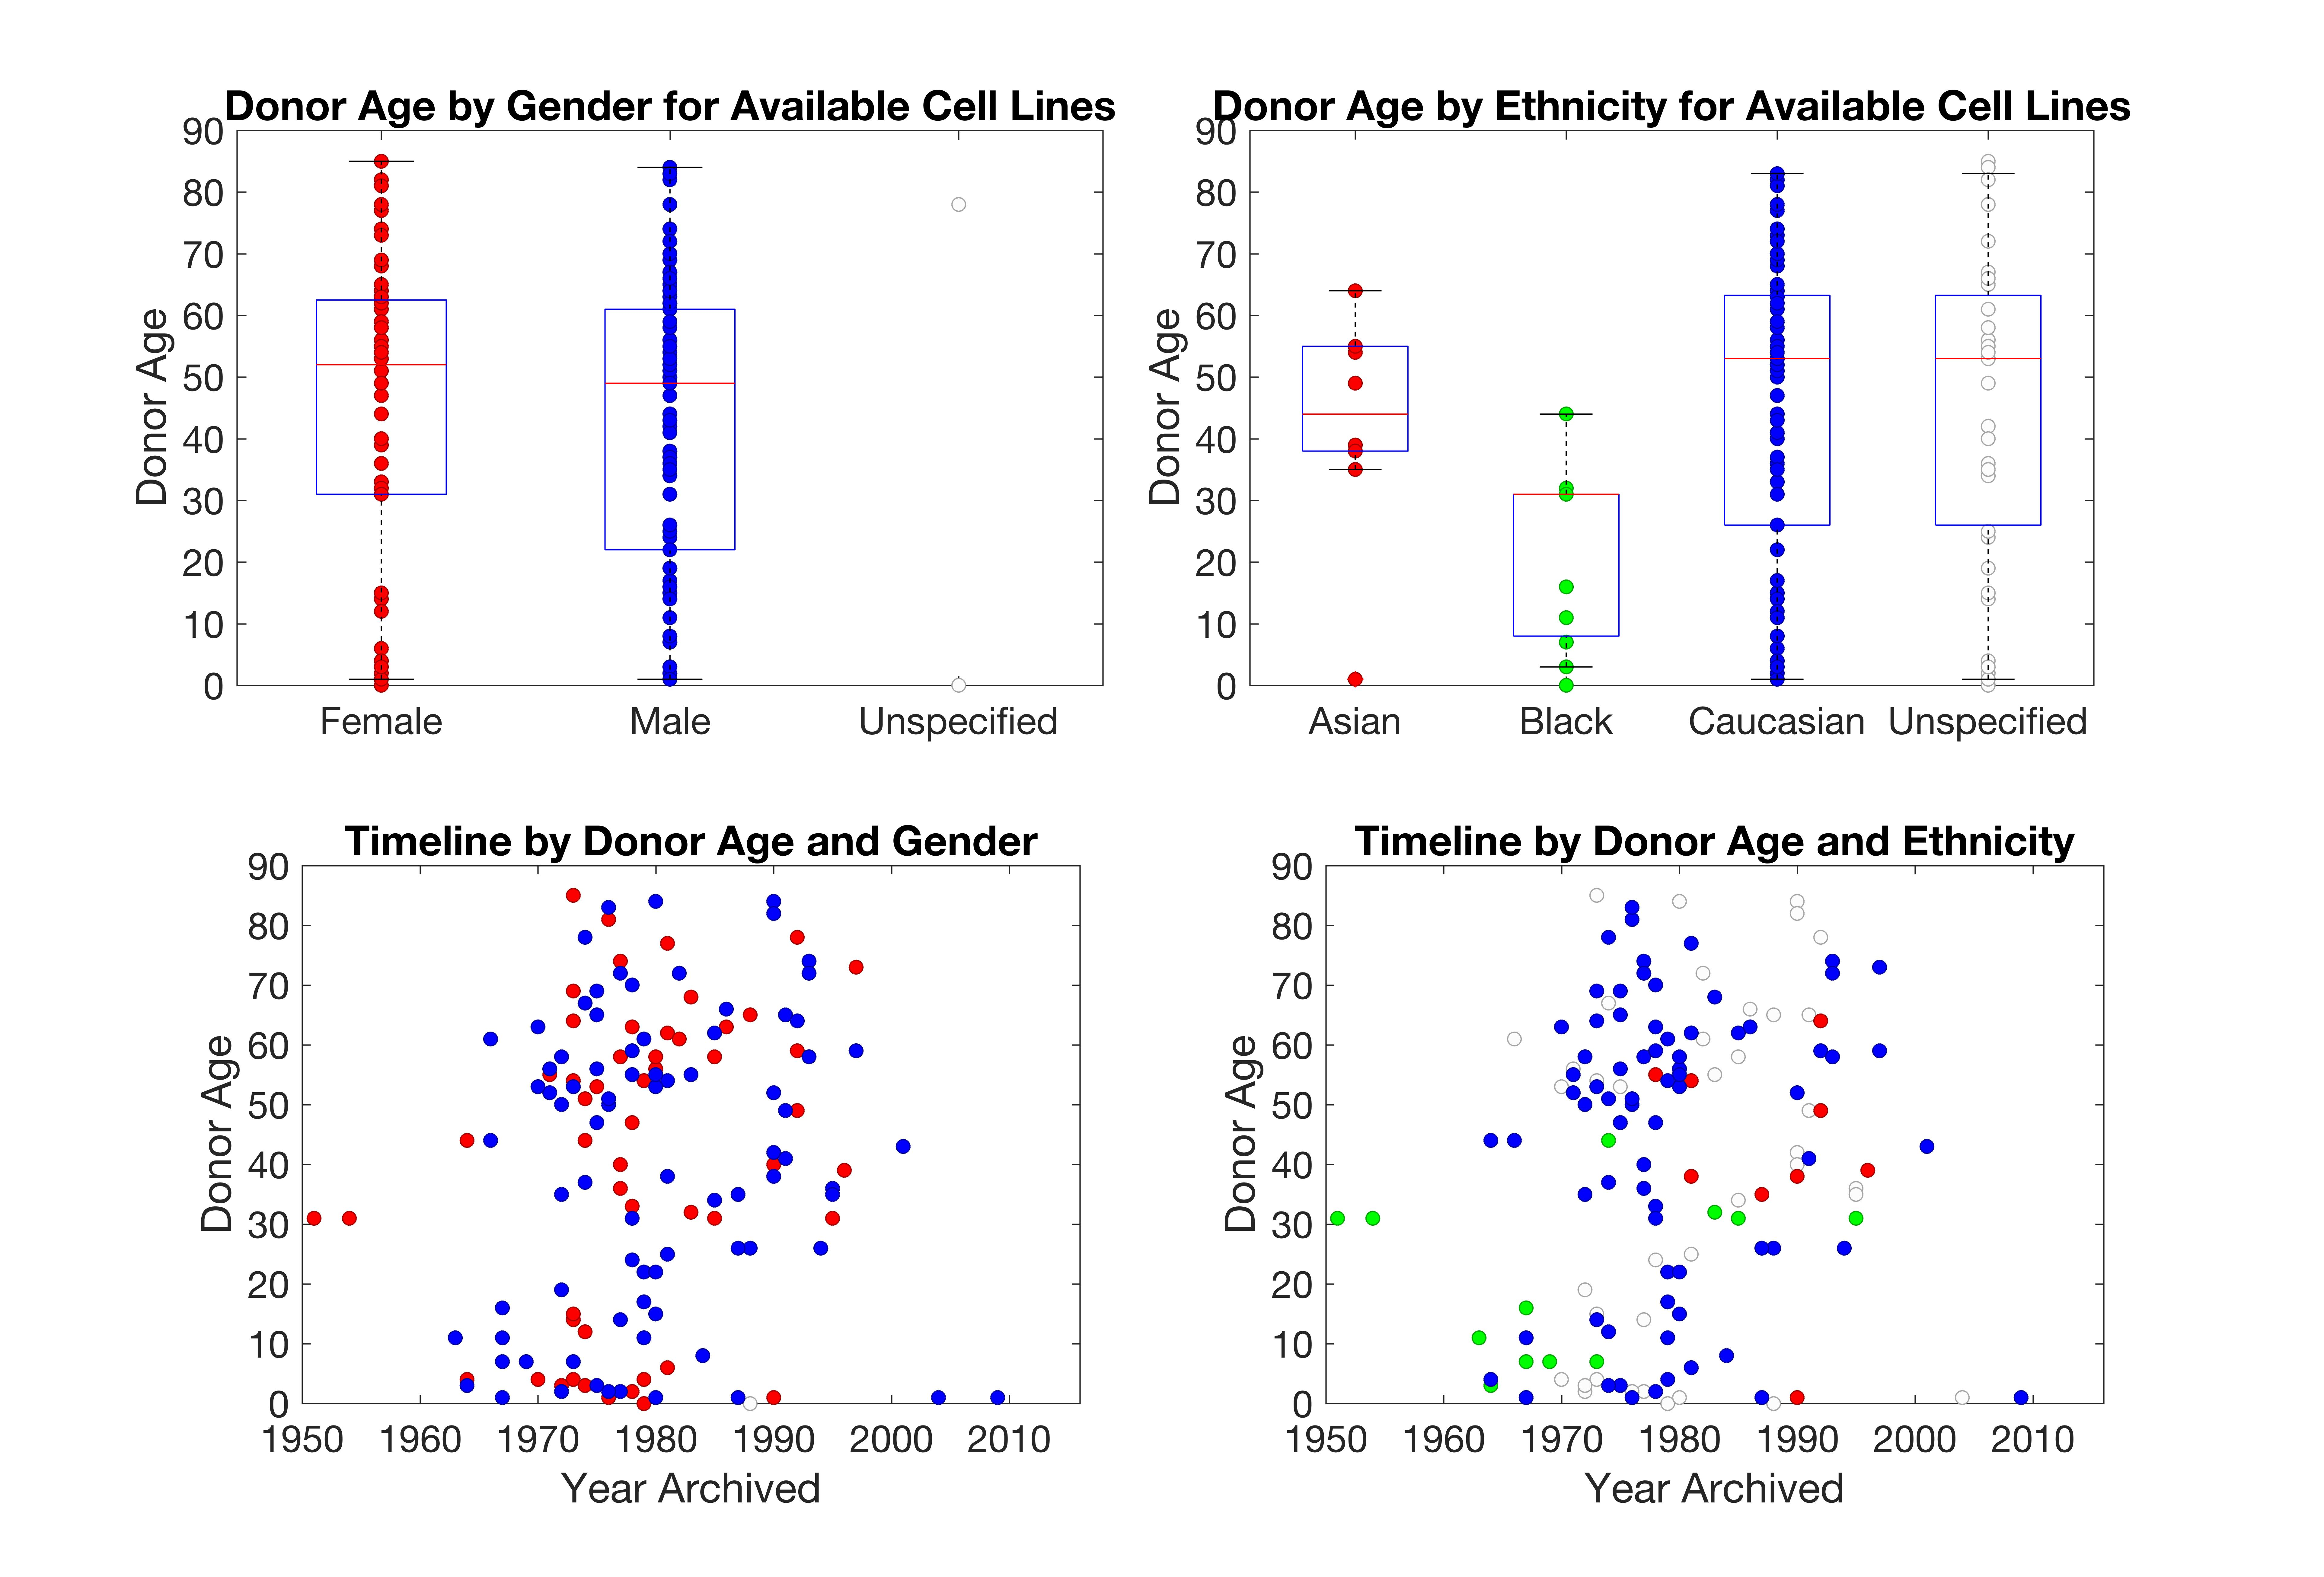
\includegraphics[width=0.98\columnwidth]{Figures/TimelineDonorAge}
\caption{\label{pcbg}Timeline of cell line introduction by donor demographics. }
\end{figure}


\begin{figure}[h!]
\centering
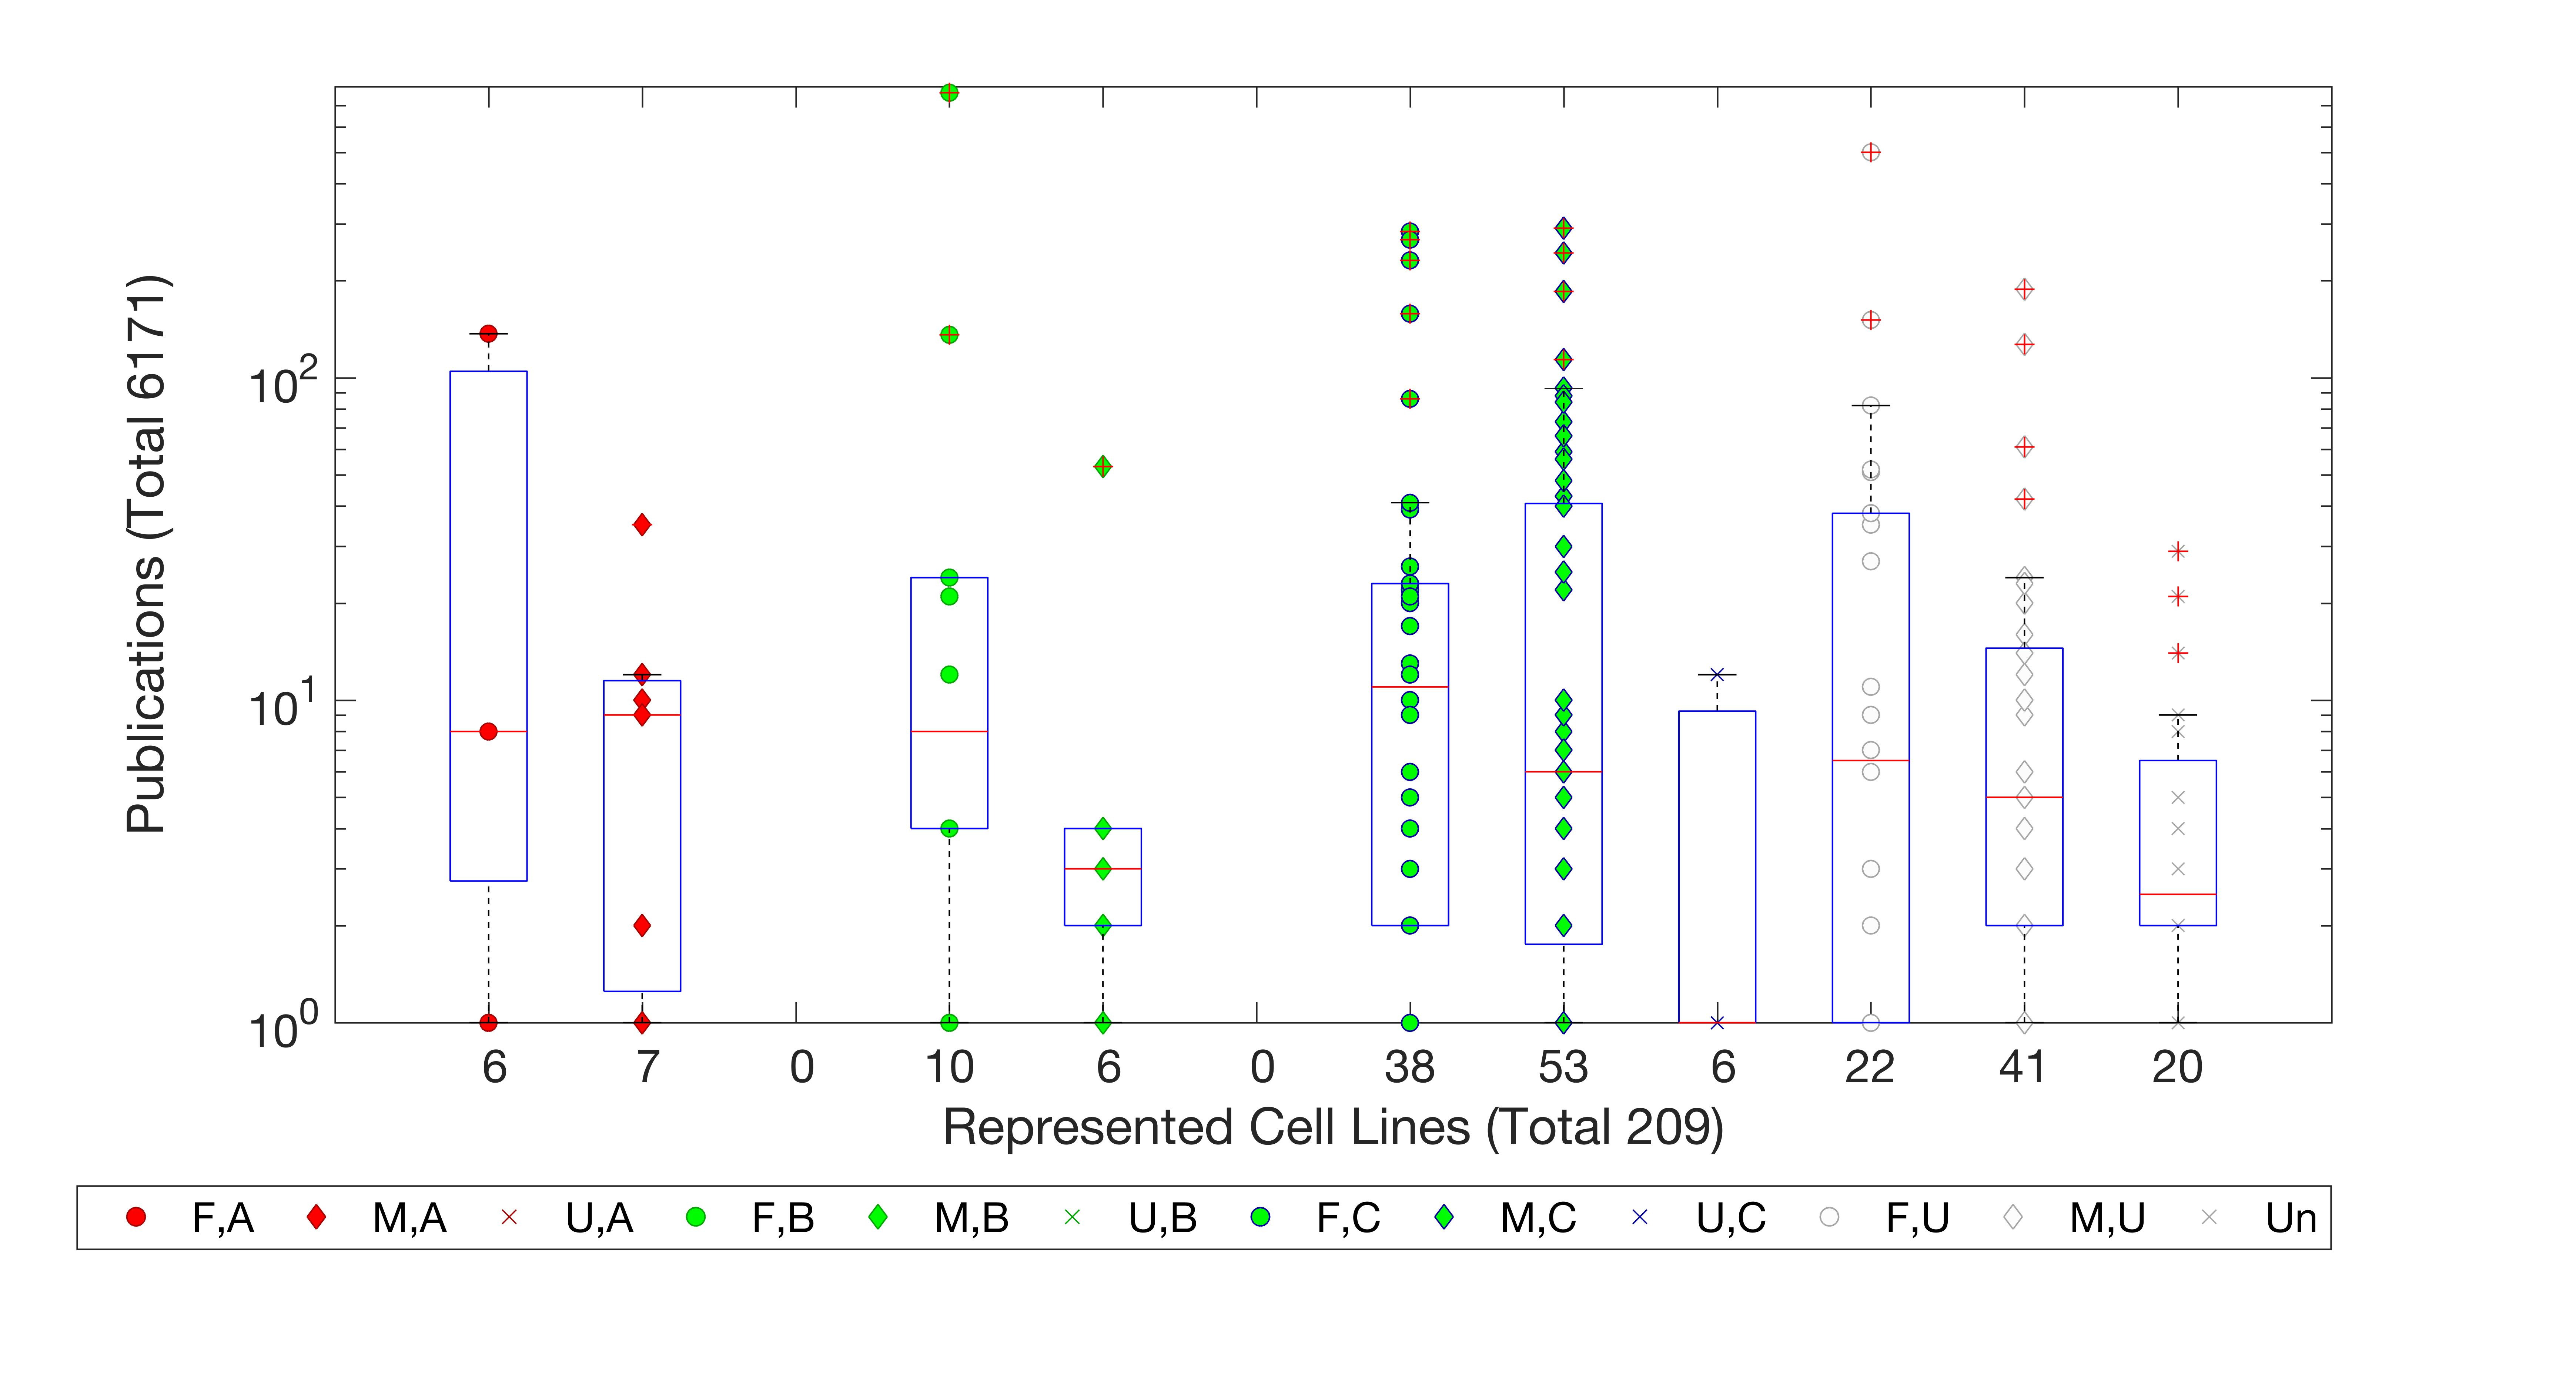
\includegraphics[width=0.98\columnwidth]{Figures/PubCountBarGraph}
\caption{\label{pcbg}Publication count for each gender and ethnicity cell line.}
\end{figure}

\begin{figure}[h!]
\centering
\includegraphics[width=0.98\columnwidth]{Figures/PubCountBarGraph_Disease}
\caption{\label{pcbg}Publication count for each gender and ethnicity cell line.}
\end{figure}

\bibliographystyle{unsrt}
\bibliography{refs}

\enddocument
